\section{其他二次曲面}\label{sec:其他二次曲面}
pbrt还支持三种曲面:\keyindex{圆锥体}{cone}{}、\keyindex{抛物面}{paraboloid}{}和\keyindex{双曲面}{hyperboloid}{}。
它们在源文件
\href{https://github.com/mmp/pbrt-v3/tree/master/src/shapes/cone.h}{\ttfamily shapes/cone.h}、
\href{https://github.com/mmp/pbrt-v3/tree/master/src/shapes/cone.cpp}{\ttfamily shapes/cone.cpp}、
\href{https://github.com/mmp/pbrt-v3/tree/master/src/shapes/paraboloid.h}{\ttfamily shapes/paraboloid.h}、
\href{https://github.com/mmp/pbrt-v3/tree/master/src/shapes/paraboloid.cpp}{\ttfamily shapes/paraboloid.cpp}、
\href{https://github.com/mmp/pbrt-v3/tree/master/src/shapes/hyperboloid.h}{\ttfamily shapes/hyperboloid.h}和
\href{https://github.com/mmp/pbrt-v3/tree/master/src/shapes/hyperboloid.cpp}{\ttfamily shapes/hyperboloid.cpp}
中实现。
我们这里不介绍它们的完整实现,
因为现在应该熟悉用于推导它们二次相交次数、参数化坐标以及偏导数的技术了。
然而,我们会简要总结这些形状的隐式和参数形式。
\reffig{3.10}是它们三种的渲染图像。
\begin{figure}[htbp]
    \centering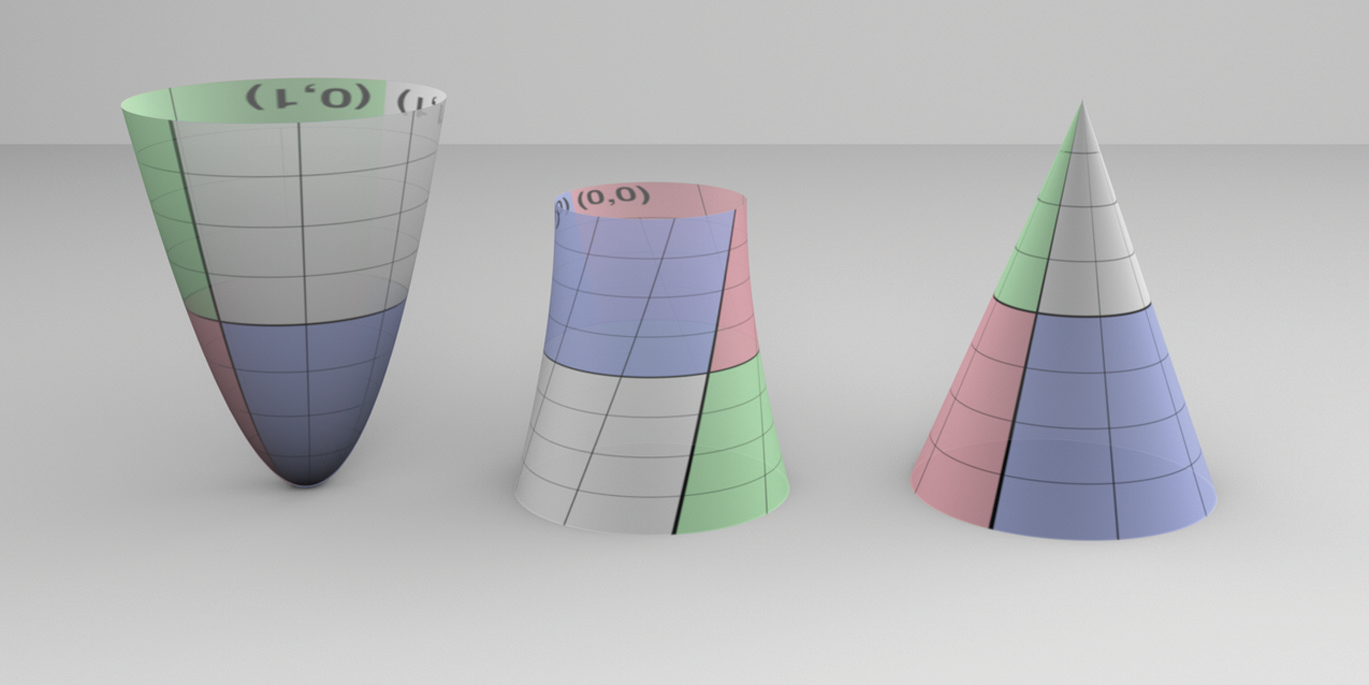
\includegraphics[width=\linewidth]{chap03/miscquads.png}
    \caption{剩下的二次曲面形状。从左到右:抛物面、双曲面和圆锥体。}
    \label{fig:3.10}
\end{figure}

\subsection{圆锥体}\label{sub:圆锥体}
以$z$轴为中心,半径为$r$高为$h$的圆锥体的隐式方程是
\sidenote{译者注:如果你理解有困难,那化为$\displaystyle\frac{x^2+y^2}{r^2}=\left(\frac{z-h}{h}\right)^2$并结合相似三角形试试吧。}
\begin{align*}
    \left(\frac{hx}{r}\right)^2+\left(\frac{hy}{r}\right)^2-(z-h)^2=0\, .
\end{align*}
圆锥体也可以参数化描述为:
\begin{align*}
    \varphi & =u\varphi_{\max}\, ,   \\
    x       & =r(1-v)\cos\varphi\, , \\
    y       & =r(1-v)\sin\varphi\, , \\
    z       & =vh\, .
\end{align*}
圆锥体上一点的偏导数为
\begin{align*}
    \frac{\partial\bm p}{\partial u} & =(-\varphi_{\max}y,\varphi_{\max}x,0)\, ,       \\
    \frac{\partial\bm p}{\partial v} & =\left(\frac{x}{v-1},\frac{y}{v-1},h\right)\, ,
\end{align*}
且二阶偏导数为
\begin{align*}
    \frac{\partial^2\bm p}{\partial u^2}         & =-\varphi_{\max}^2(x,y,0)\, ,           \\
    \frac{\partial^2\bm p}{\partial u\partial v} & =\frac{\varphi_{\max}}{1-v}(y,-x,0)\, , \\
    \frac{\partial^2\bm p}{\partial v^2}         & =(0,0,0)\, .
\end{align*}

\subsection{抛物面}\label{sub:抛物面}
以$z$轴为中心,半径为$r$高为$h$的抛物面的隐式方程是
\sidenote{译者注:如果你理解有困难,那化为$\displaystyle\frac{x^2+y^2}{r^2}=\frac{z}{h}$试试吧。}
\begin{align*}
    \frac{hx^2}{r^2}+\frac{hy^2}{r^2}-z=0\, ,
\end{align*}
且它的参数形式为
\begin{align*}
    \varphi & =u\varphi_{\max}\, ,                   \\
    z       & =v(z_{\max}-z_{\min})\, ,              \\
    r       & =r_{\max}\sqrt{\frac{z}{z_{\max}}}\, , \\
    x       & =r\cos\varphi\, ,                      \\
    y       & =r\sin\varphi\, .
\end{align*}
偏导数为
\begin{align*}
    \frac{\partial\bm p}{\partial u} & =(-\varphi_{\max}y,\varphi_{\max}x,0)\, ,                        \\
    \frac{\partial\bm p}{\partial v} & =(z_{\max}-z_{\min})\left(\frac{x}{2z},\frac{y}{2z},1\right)\, ,
\end{align*}
以及
\begin{align*}
    \frac{\partial^2\bm p}{\partial u^2}         & =-\varphi_{\max}^2(x,y,0)\, ,                                                   \\
    \frac{\partial^2\bm p}{\partial u\partial v} & =\varphi_{\max}(z_{\max}-z_{\min})\left(-\frac{y}{2z},\frac{x}{2z},0\right)\, , \\
    \frac{\partial^2\bm p}{\partial v^2}         & =-(z_{\max}-z_{\min})^2\left(\frac{x}{4z^2},\frac{y}{4z^2},0\right)\, .
\end{align*}

\subsection{双曲面}\label{sub:双曲面}
最后,双曲面的隐式形式为
\sidenote{译者注:原文写成了双叶双曲面方程,但下文参数形式为单叶双曲面方程。此处为了一致性已做修改。}
\begin{align*}
    x^2+y^2-z^2=1\, ,
\end{align*}
且它的参数形式为
\sidenote{译者注:可以理解为过点$(x_1,y_1,z_1)$和$(x_2,y_2,z_2)$的直线段绕$z$轴旋转扫掠生成双曲面。}
\begin{align*}
    \varphi & =u\varphi_{\max}\, ,               \\
    x_r     & =(1-v)x_1+vx_2\, ,                 \\
    y_r     & =(1-v)y_1+vy_2\, ,                 \\
    x       & =x_r\cos\varphi-y_r\sin\varphi\, , \\
    y       & =x_r\sin\varphi+y_r\cos\varphi\, , \\
    z       & =(1-v)z_1+vz_2\, .
\end{align*}
偏导数为
\begin{align*}
    \frac{\partial\bm p}{\partial u} & =(-\varphi_{\max}y,\varphi_{\max}x,0)\, ,                                                          \\
    \frac{\partial\bm p}{\partial v} & =((x_2-x_1)\cos\varphi-(y_2-y_1)\sin\varphi,(x_2-x_1)\sin\varphi+(y_2-y_1)\cos\varphi,z_2-z_1)\, ,
\end{align*}
以及
\begin{align*}
    \frac{\partial^2\bm p}{\partial u^2}         & =-\varphi_{\max}^2(x,y,0)\, ,                                                                      \\
    \frac{\partial^2\bm p}{\partial u\partial v} & =\varphi_{\max}\left(-\frac{\partial p_y}{\partial v},\frac{\partial p_x}{\partial v},0\right)\, , \\
    \frac{\partial^2\bm p}{\partial v^2}         & =(0,0,0)\, .
\end{align*}